% chapters/glitch-gp.tex
%
% Copyright 2023 Alexander Lyttle.
%
% This work may be distributed and/or modified under the conditions of the
% LaTeX Project Public License (LPPL) version 1.3 or later.
%
% The latest version of this license is in
% https://www.latex-project.org/lppl.txt and version 1.3 or later is part of
% all distributions of LaTeX version 2005/12/01 or later.
%
%
\chapter[Modelling Acoustic Glitches with a Gaussian Process]{Modelling Acoustic Glitch Signatures in Stellar Oscillations with a Gaussian Process}\label{chap:glitch-gp}

\textit{In this chapter, I apply a new method for modelling acoustic glitch signatures in the radial mode frequencies of solar-like oscillators. I compare my method to another using a model star with different levels of noise. Then, I apply both methods to the star 16 Cyg A. I show that my method can be used to find the strength and location of glitches caused by the second ionisation of helium and the base of the convective zone. I also demonstrate that my method improves treatment of the smoothly varying component of the mode frequencies.}

\section{Introduction}

Let us consider a non-rotating star which oscillates at frequencies \(\nu_{nl}\), where \(n\) and \(l\) are the radial order and angular degree of the modes. We may model the modes as the sum of a smoothly-varying component, \(\tilde{f}(n, l)\), and quickly-varying, small change in frequency, \(\delta\nu_{nl}\), arising from glitches in the stellar structure,
%
\begin{equation}
    f(n, l) = \tilde{f}(n, l) + \delta\nu_{nl},\label{eq:general-glitch}
\end{equation}
%
where \(\delta\nu_{nl}\) is some function of frequency which may be evaluated at \(\tilde{f}(n, l)\).

In principle, \(\delta\nu\) could arise from any glitches expected in a particular star. Here, we consider glitches in main sequence solar-like oscillators. In Chapter \ref{chap:glitch}, we derived approximations for \(\delta\nu_{nl}\) arising from acoustic glitches caused by the second ionisation of helium and the BCZ. We choose to ignore contributions to \(\delta\nu_{nl}\) from the first ionisation of helium. Consequently, we let \(\delta\nu_{nl} = \delta\nu_\helium + \delta\nu_\bcz\) where each component depends on parameters relating to properties of the glitches (cf. Equations \ref{eq:he-osc} and \ref{eq:bcz-osc}),
%
\begin{align}
    \delta\nu_\helium &= \alpha_\helium \nu_0 \nu \, \ee^{-\beta_\helium \nu^2} \sin(4\pi\tau_\helium\nu + \phi_\helium), \label{eq:he-glitch}\\
    \delta\nu_\bcz &= \alpha_\bcz \nu_0 \nu^{-2} \, \sin(4\pi\tau_\bcz\nu + \phi_\bcz). \label{eq:bcz-glitch}
\end{align}
%
The parameters \(\alpha_\helium \simeq \Gamma_\heII\) and \(\beta_\helium \propto \Delta_\heII^2\) relate to the area and variance of the Gaussian-like depression in \(\gamma\) caused by the second ionisation of helium (see Equation \ref{eq:he-gamma}). The amplitude parameter for the BCZ glitch is proportional to the difference in the second density derivative at the base of the convective zone (\(\alpha_\bcz \propto \Delta_{\bcz}\)) with units of frequency squared. The approximate acoustic depths of second helium ionisation and the BCZ are given by \(\tau_\helium\) and \(\tau_\bcz\) respectively, and \(\phi_\helium\) and \(\phi_\bcz\) are arbitrary phase constants.

Providing \(\tilde{f}(n, l)\) is a good approximation of the mode frequencies, we can calculate \(\delta\nu_{nl}\) at \(\tilde{f}(n, l)\) to predict \(f(n, l)\). For example, \(\tilde{f}(n,l)\) could be a \(K\)-th order polynomial in \(n\) with coefficients \(a_{lk}\) \citep[e.g.][]{Kjeldsen.Bedding.ea2005,Ulrich1986},
%
\begin{equation}
    \tilde{f}(n, l) = \nu_0 \sum_{k=0}^{K} a_{lk} n^k. \label{eq:poly}
\end{equation}
%
The linear component of this is equivalent to the asymptotic expression (see Equation \ref{eq:asy}) and the remaining terms describe curvature in the mode frequencies. However, there are drawbacks to using a polynomial for \(\tilde{f}(n, l)\). Whilst a polynomial with \(K = \infty\) can represent any function, this is impractical here. If \(K\) is too low, then it will not be flexible enough, biasing the inference of \(\delta\nu_\helium\) and \(\delta\nu_\bcz\). Yet, if \(K\) is too high, then the model will over-fit and the glitch component may be missed. Regularising the polynomial is one solution to over-fitting, but this adds extra parameters to tune. Additionally, a finite polynomial represents only a small fraction of function space, systematically biasing our model to a particular functional form of \(\tilde{f}\).

\defcitealias{Verma.Raodeo.ea2019}{V19}

Directly fitting the glitch the above way has been done before \citep[e.g.][]{Verma.Faria.ea2014,Verma.Raodeo.ea2017,Mazumdar.Monteiro.ea2014}. In this work, we will compare the most recent version of this method \citep[][hereafter V19]{Verma.Raodeo.ea2019} with a new method. Our method will make use of a Gaussian Process (GP) to marginalise over the uncertainty in the functional form of \(f\). In the next section, we introduce the data used in comparing the two methods. Then, we define both modelling in Section \ref{sec:glitch-methods}. Finally, we apply the methods to the data and present the results and discussion in Sections \ref{sec:glitch-results} and \ref{sec:glitch-disc} respectively.

\section{Data}\label{sec:glitch-data}

In this section, we briefly outline the data used to compare our new method with the \citetalias{Verma.Raodeo.ea2019} method. For simplicity, we only use observations of radial mode frequencies in this work. However, both methods can be extended to use higher-degree modes.

\begin{table}
    \centering
    \caption[Observations of radial mode frequency \(\nu_n\) at radial order \(n\) for model star S and 16 Cyg A.]{Observations of radial mode frequency \(\nu_n\) at radial order \(n\) for model star S (\emph{left}) and 16 Cyg A (\emph{right}). \(N\) are the number of observed radial orders and the scale of the Gaussian noise added to each column is given by \(\sigma_\obs\) where appropriate. The values and their uncertainties for 16 Cyg A come from \citet{Lund.SilvaAguirre.ea2017}.}
    \label{tab:glitch-obs}
    \begin{tabular}{ccccc}
\toprule
Case & Worst & Better & Best & Truth \\
$N, \sigma_n$ & 6, 1.00 & 12, 0.10 & 18, 0.01 &  \\
$n$ &  &  &  &  \\
\midrule
12 & --- & --- & 1781.726 & 1781.729 \\
13 & --- & --- & 1914.348 & 1914.330 \\
14 & --- & --- & 2047.296 & 2047.314 \\
15 & --- & 2180.16 & 2180.107 & 2180.125 \\
16 & --- & 2312.00 & 2312.030 & 2312.029 \\
17 & --- & 2442.64 & 2442.807 & 2442.808 \\
18 & 2577.2 & 2574.32 & 2574.260 & 2574.263 \\
19 & 2706.4 & 2706.50 & 2706.612 & 2706.596 \\
20 & 2839.0 & 2839.46 & 2839.446 & 2839.476 \\
21 & 2971.5 & 2972.92 & 2972.718 & 2972.727 \\
22 & 3107.4 & 3105.77 & 3105.749 & 3105.759 \\
23 & 3240.0 & 3239.18 & 3239.177 & 3239.175 \\
24 & --- & 3372.94 & 3372.980 & 3372.990 \\
25 & --- & 3507.22 & 3507.115 & 3507.112 \\
26 & --- & 3641.56 & 3641.715 & 3641.702 \\
27 & --- & --- & 3776.339 & 3776.350 \\
28 & --- & --- & 3911.281 & 3911.279 \\
29 & --- & --- & 4046.319 & 4046.312 \\
\bottomrule
\end{tabular}

\end{table}

\begin{figure}[tb]
    \centering
    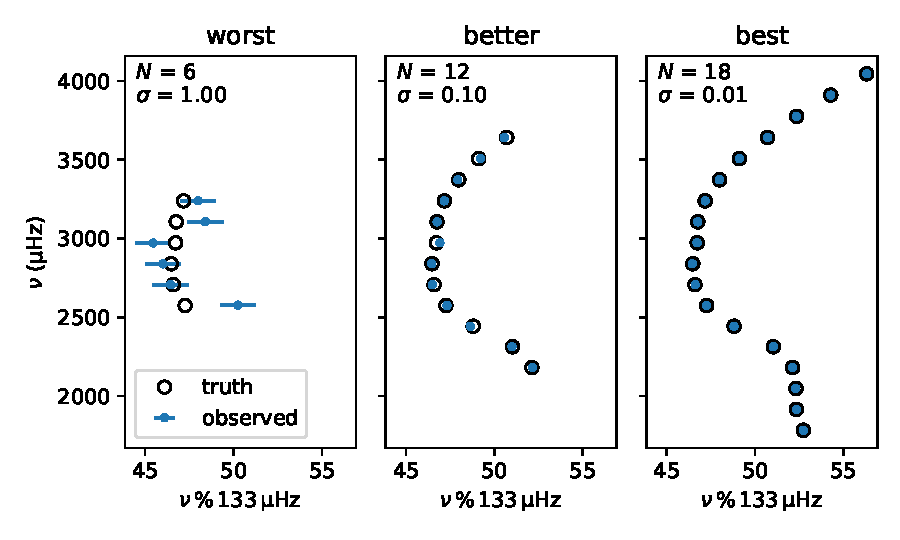
\includegraphics{figures/glitch-test-obs.pdf}
    \caption{Echelle plot of simulated true and `observed' radial mode frequency data from model star S for worst, better, and best case scenarios.}
    \label{fig:glitch-test-obs}
\end{figure}

\paragraph{Test Star} We created three sets of test data for worst, better, and best case scenarios using stellar model R (defined in Section \ref{sec:model-s}). Model R is similar to the Sun, with surface parameters of \(\teff = \SI{5682}{\kelvin}\), \(\log g = 4.426\) and \([\mathrm{Fe/H}] = 0.03\), and bulk parameters of \(M = \SI{1.00}{\solarmass}\), \(R = \SI{1.01}{\solarmass}\) and \(t_\star = \SI{4.07}{\giga\year}\). We calculated radial order modes (\(l=0\)) for the test star using the \textsc{GYRE} oscillation code \citep{Townsend.Teitler2013}. Then, we selected different numbers of modes (\(N\)) symmetrically about a reference frequency, \(\nu_\mathrm{ref} = \SI{2900}{\micro\hertz}\) (close to the expected frequency at maximum power of the star). To the frequencies, we added Gaussian noise scaled by \(\sigma_\obs = 1.0\), \(0.1\), and \SI{0.01}{\micro\hertz}, for the worst, better, and best cases respectively. The parameters and mode frequencies for each test case are shown in Table \ref{tab:glitch-obs}. We also plotted the modes on an echelle diagram in Figure \ref{fig:glitch-test-obs}. We can see the effect of the helium glitch in the echelle diagrams, where there is a periodic feature which is strongest at low frequencies. The glitch signature is visible in the better case and clearest in the best case scenario.

\paragraph{16 Cyg A} We used the asteroseismic benchmark star 16 Cyg A as an example real star to test both methods. We adopted values for 16 radial mode frequencies identified by \citet{Lund.SilvaAguirre.ea2017} using observations from \emph{Kepler} \citep[][KIC 12069424]{Borucki.Koch.ea2010}. The mode frequencies and their associated uncertainties are given in Table \ref{tab:glitch-obs}. The glitch has been previously studied for 16 Cyg A with its binary companion 16 Cyg B in \citet{Verma.Faria.ea2014}, making it a useful subject for comparison. Similarly to model R, this target is a solar analogue. However, it is slightly hotter, more evolved and more metal-rich, with \(\teff = \SI{5825(50)}{\kelvin}\), \(\log g = \SI{4.33(7)}{\dex}\) and \([\mathrm{Fe/H}] = \SI{0.10(3)}{\dex}\) \citep{Ramirez.Melendez.ea2009}. Its fundamental stellar parameters are \(M \approx \SI{1.1}{\solarmass}\), \(R \approx \SI{1.2}{\solarradius}\) and \(t_\star \approx \SI{7}{\giga\year}\) \citep{SilvaAguirre.Lund.ea2017}.

\section{Methods}\label{sec:glitch-methods}

In this section, we describe the two models for radial mode frequency, \(\nu_n = f(n, 0)\), and the fitting methods being compared in this work. The first is the \citetalias{Verma.Raodeo.ea2019} method, originally used in \citet{Verma.Faria.ea2014} to study the 16 Cyg binary star system. Secondly, we introduce our new `GP method'. Both methods use different statistical philosophy and formulation of the smoothly varying component, \(\tilde{f}(n)\). However, they each fit the same glitch component \(\delta\nu = \delta\nu_\helium + \delta\nu_\bcz\) as given in Equations \ref{eq:he-glitch} and \ref{eq:bcz-glitch}.

\subsection{The V19 Method}

The \citetalias{Verma.Raodeo.ea2019} method is a specific case of Equation \ref{eq:general-glitch}, where the smooth component is approximated by 4-th order polynomial,
%
\begin{equation}
    f_A(n) = \tilde{f}_A(n) + \delta\nu_\helium + \delta\nu_\bcz; \quad \tilde{f}_A(n) = \sum_{k=0}^{4} b_k n^k,
\end{equation}
%
\sloppy where \(b_k \equiv a_{0k} \nu_0\) from Equation \ref{eq:poly}. The model parameters are given by \(\vect{\theta}_A = (b_0, \dots, b_4, a_\helium, \beta_\helium, \tau_\helium, \phi_\helium, a_\bcz, \tau_\bcz, \phi_\bcz)\), where the glitch amplitude parameters are modified to include \(\nu_0\) such that \(a_i \equiv \alpha_i\nu_0\). The \(\nu_0\) parameter is not explicitly included in the \citetalias{Verma.Raodeo.ea2019} model, but we find it useful to keep the scaling in mind, and we use \(\nu_0\) in the GP model. 

The model parameters are optimised by minimising a \(\chi^2\) cost function with a regularisation term,
%
\begin{equation}
    \chi^2 = \sum_n \left[ \frac{\nu_n^\obs - f_{A}(n)}{\sigma_n^\obs} \right]^2 + \lambda^2 \sum_n \left[ \frac{\dd^3}{\dd n^3} \tilde{f}_A(n)\right]^2,
\end{equation}
%
where \(\nu_n^\obs\) and \(\sigma_n^\obs\) are the observed mode and its uncertainty at radial order \(n\), and \(\lambda\) is the regularisation parameter. The regularisation was used to avoid the polynomial over-fitting and absorbing the glitch terms.

We fitted the model using the \textsc{GlitchPy} code\footnote{\url{https://github.com/alexlyttle/GlitchPy}, adapted from \url{https://github.com/kuldeepv89/GlitchPy}.}. The fitting method is described in \citet{Verma.Raodeo.ea2019}, in which we adopted the same value of \(\lambda=7\) and bounds for the selection of initial parameters. We chose the initial parameters randomly within their bounds and optimised them using a BFGS minimisation of \(\chi^2\) \citep{Fletcher1987}, repeated 200 times until a global minimum was found. We further repeated this for 1000 realisations of the observed \(\nu_n\) with Gaussian noise scaled by \(\sigma_n^\obs\) to obtain a range of possible solutions.

\subsection{The GP Method}

In the second method, we used a Gaussian Process \citep[GP; see][for a recent review]{Aigrain.Foreman-Mackey2022} instead of a high-order polynomial to model the smoothly varying component of the mode frequencies. The GP represents a probability distribution in function-space, meaning that we can quantify the uncertainty associated with the functional form of $f$. We write our model for a set of modes \(\vect{n} = \{n_i\}_{i=1}^N\) as a random draw from a GP,
%
\begin{equation}
    f_{B}(\vect{n}) \sim \mathcal{GP}\left[ m(\vect{n}), k(\vect{n}, \vect{n}') \right],%\text{\footnotemark}
\end{equation}
%
% \footnotetext{In this section we use the convention that some random variable \(y\) drawn from a distribution \(q\) given parameters \(x\) may be written as \(y \sim q(x)\).}%
where \(m\) and \(k\) are the mean and kernel functions, and \(\vect{n}'\) is any other set of radial orders, \(\vect{n}' = \{n'_j\}_{j=1}^M\). The mean function describes where we expect \(\nu_n\) to be given some approximate physical reasoning. Therefore, we define our mean function for any \(n\)-th order mode as,
%
\begin{equation}
    m(n) = \tilde{f}_B(n) + \delta\nu_\helium + \delta\nu_\bcz; \quad \tilde{f}_B(n) = (n + \varepsilon) \nu_0, \label{eq:asy-glitch}
\end{equation}
%
where \(\tilde{f}_B(n)\) is the asymptotic approximation of the mode frequency (see Equation \ref{eq:asy}).

The kernel represents the expected covariance between the values of the function at different \(n\). We chose the squared exponential kernel function to be compatible with a smoothly-varying function of \(n\). Evaluating the kernel gives an \(N \times M\) matrix with an element \((i,j)\) given by,
%
\begin{equation}
    k(n_i, n'_j) = \alpha_k \nu_0 \, \ee^{- (n_i - n'_j)^2 / 2\lambda_k^2},
\end{equation}
%
where \(\alpha_k\) is a dimensionless amplitude scale factor and \(\lambda_k\) is the length scale (in units of radial order). Both kernel parameters control the flexibility of the GP. The amplitude parameter scales the covariance and \(\lambda_k\) describes the breadth of correlation between different modes. As \(\lambda_k \rightarrow 0\), the off-diagonal terms of the kernel approach zero producing uncorrelated noise with a variance of \(\alpha_k\nu_0\). We found values of \(\alpha_k = 0.5\) and \(\lambda_k = 5\) predicted smoothly varying functions compatible with our prior expectation.

The GP likelihood for some set of observations \(\vect{\nu}_\obs = \{\nu_{n_i}^\obs\}_{i=1}^N\) is a multivariate normal distribution centred on the mean function with covariance provided by the kernel function. We also added Gaussian noise terms to the diagonal of the covariance matrix,
%
\begin{equation}
    \vect{\nu}_\obs \sim \mathcal{N}\left( \vect{\mu}, \,  \vect{\Sigma} \right); \quad \vect{\Sigma} = \vect{K} + \mathrm{diag}(\sigma^2 + \vect{\sigma}_\obs^2), \label{eq:gp-like}
\end{equation}
%
where \(\vect{\mu} = m(\vect{n})\) and \(\vect{K} = k(\vect{n}, \vect{n})\). The scales of Gaussian noise in the model and observations are \(\sigma\) and \(\vect{\sigma}_\obs\) respectively. We included \(\sigma\) to account for uncorrelated noise in the model, for example from the difference between \(\delta\nu\) evaluated at \(\tilde{f}_B(n)\) and at the `true' mode frequencies.

To make noiseless predictions of mode frequencies \(\vect{\nu}_\star\) at new radial orders \(\vect{n}_\star\), we drew from the following multivariate normal distribution \citep{Rasmussen.Williams2006},
%
\begin{equation}
    \vect{\nu}_\star \mid \vect{\nu}_\obs \sim \mathcal{N} \left[ \vect{\mu}_\star + \vect{K}_\star^\mathsf{T} \, \vect{\Sigma}^{\,-1} \, (\vect{\nu}_\obs - \vect{\mu}), \, \vect{K}_{\star\star} - \vect{K}_\star^\mathsf{T} \, \vect{\Sigma}^{\,-1} \, \vect{K}_\star \right]
\end{equation}
%
where,
%
\begin{equation*}
    \vect{\mu}_\star = m(\vect{n}_\star), \quad \vect{K}_\star = k(\vect{n}, \vect{n}_\star), \quad \vect{K}_{\star\star} = k(\vect{n}_\star, \vect{n}_\star).
\end{equation*}
%
% This satisfies the consistency requirement that GP must specify any mode \(\nu_n \sim \mathcal{N}(\mu_n, K_{nn})\) where \(K_{nn}\) is the sub-matrix of the covariance of 

We used Bayes' theorem (see Equation \ref{eq:bayes-theorem}) to estimate the probability of our model parameters, \(\vect{\theta}_B = (\nu_0, \varepsilon, \alpha_\helium, \beta_\helium, \tau_\helium, \phi_\helium, a_\bcz, \tau_\bcz, \phi_\bcz, \sigma)\), given observations of mode frequencies. Hence, we write the posterior probability density as,
%
\begin{equation}
    p(\vect{\theta}_B \mid \vect{\nu}_\obs) = \frac{p(\vect{\nu}_\obs \mid \vect{\theta}_B)\,p(\vect{\theta}_B)}{p(\vect{\nu}_\obs)} \equiv \frac{\mathcal{L}(\vect{\theta}_B)\,p(\vect{\theta}_B)}{\mathcal{Z}},
\end{equation}
%
where \(\mathcal{L}(\vect{\theta}_B)\) is the likelihood of the data given the model, \(p(\vect{\theta}_B)\) is the prior probability density of the model parameters, and \(\mathcal{Z}\) is the `evidence' (or normalisation). The true posterior density function cannot be derived analytically, so we estimated it with the `nested sampling' algorithm \citep{Skilling2004}. By evaluating the prior volume at contours of constant likelihood, nested sampling estimates \(\mathcal{Z}\) to weight samples according to their posterior probability. This method requires functions for the log-likelihood and a transform which maps random samples in the unit hypercube to prior parameter space. 

\begin{table}
    \centering
    % \caption{The mean and variance for the prior normal distributions on each parameter where values are not explicitly given in the text.}
    \caption[The GP model parameters and their prior distributions.]{The GP model parameters and their prior distributions. Normal distributions are parametrised by the mean and variance (i.e. \(\mathcal{N}(\mu,\sigma^2)\)). Uniform distributions are parametrised by their lower and upper bounds.}
    \label{tab:glitch-prior}
    \begin{tabular}{lll}
\toprule
Parameter & \multicolumn{2}{c}{Prior} \\
\midrule
 & Test Star & 16 Cyg A \\
\midrule
$\nu_0/\si{\micro\hertz}$ & $\mathcal{N}(132.8,0.01)$ & $\mathcal{N}(103.28,0.0025)$ \\ 
$\varepsilon$ & $\mathcal{N}(1.4,0.0025)$ & $\mathcal{N}(1.45,0.0025)$ \\ 
$\ln(\alpha_\mathrm{cz}/\si{\micro\hertz\squared})$ & $\mathcal{N}(8.29,0.64)$ & $\mathcal{N}(8.04,0.64)$ \\ 
$\ln(\alpha_\mathrm{He}/\si{\mega\second})$ & $\mathcal{N}(-11.1,0.04)$ & $\mathcal{N}(-10.85,0.04)$ \\
$\ln(\beta_\mathrm{He}/\si{\mega\second\squared})$ & $\mathcal{N}(-15.07,0.16)$ & $\mathcal{N}(-14.56,0.16)$ \\
$\ln(\tau_\mathrm{cz}/\si{\mega\second})$ & $\mathcal{N}(-6.09,0.04)$ & $\mathcal{N}(-5.84,0.04)$ \\
$\ln(\tau_\mathrm{He}/\si{\mega\second})$ & $\mathcal{N}(-7.19,0.04)$ & $\mathcal{N}(-6.94,0.04)$ \\
$\ln(\sigma/\si{\micro\hertz})$ & $\mathcal{N}(- 4.605, 4)$ & $\mathcal{N}(- 4.605, 4)$ \\
$\phi_\helium, \phi_\bcz$ & $\mathcal{U}(0, 2\pi)$ & $\mathcal{U}(0, 2\pi)$ \\
\bottomrule
\end{tabular}

\end{table}

Following Equation \ref{eq:gp-like}, we defined the log-likelihood of the model as,
%
\begin{equation}
    \ln\mathcal{L}_B = - \frac12 \left[ {(\vect{\nu}_\obs - \vect{\mu})^\mathsf{T} \vect{\Sigma}^{\,-1} (\vect{\nu}_\obs - \vect{\mu})} + \ln(| \vect{\Sigma} |) + N\ln(2 \pi) \right],
\end{equation}
%
where \(\vect{\mu}\) and \(\vect{\Sigma}\) depend on \(\vect{\theta}_B\). The prior transform for \(\vect{\theta}_B\) is the inverse cumulative distribution function associated with the prior distribution \(p(\vect{\theta}_B)\). We treated the prior for each of \(\vect{\theta}_B\) independently. The total prior distribution is the product of distributions for each parameter, \(p(\vect{\theta}_B) = \prod_j p(\theta_{j})\). We give the prior distributions and their shape parameters in Table \ref{tab:glitch-prior}. In the following paragraphs, we justify our choice of prior distributions based on approximate scaling relations between the parameters. % We also summarise the prior distributions and their parameters in Table \todo{Table summary}

\paragraph{Smooth Component} Starting with priors for the parameters in \(\tilde{f}_B(n)\), we chose normal distributions,
%
\begin{gather}
    \nu_0 \sim \mathcal{N}(\overline{\nu}_0, s_{\nu_0}^2), \quad \varepsilon \sim \mathcal{N}(\overline{\varepsilon}, s_\varepsilon^2),%\\
    % \phi_\helium, \phi_\bcz \sim \mathcal{U}\left(0, 2\pi\right),
\end{gather}
%
centred on \(\overline{\nu}_0\) and \(\overline{\varepsilon}\) and scaled by \(s_{\nu_0}\) and \(s_\varepsilon\). For example, the location and scale parameters could come from global estimates of \(\langle\Delta\nu_n\rangle\) or a linear fit to the modes. We determined \(\overline{\nu}_0\) and \(\overline{\varepsilon}\) for the test stars from a linear fit to the true mode frequencies, and added representative uncertainties of 10 and 5 per cent respectively. For 16 Cyg A, we used measurements of \(\langle\Delta\nu_n\rangle\) and \(\nu_{\max}\) from \citet{Lund.SilvaAguirre.ea2017} to estimate \(\overline{\nu}_0\) and \(\overline{\varepsilon}\).

% Priors for the following parameters follow a log-normal distribution to ensure they are positive. We also exploit the property that the scale of a normal distribution in natural log-space is approximately the scale in real-space as a fraction of the distribution mean.

\paragraph{Acoustic Depths} We derived a prior on \(\tau_\helium\) and \(\tau_\bcz\) by observing how they scale with acoustic radius (\(\tau_0\)) in the grid of stellar models from \citet{Lyttle.Davies.ea2021} and the results of \citet{Verma.Rorsted.ea2022}. Typically, the fractional depth of He\,\textsc{ii} ionisation and the BCZ are \(\tau_\heII/\tau_0 \approx 0.2\) and \(\tau_\bcz/\tau_0 \approx 0.6\), for main sequence solar-like oscillators (see, e.g. Figure \ref{fig:gamma-sound-speed}). We formed the prior distributions from these relations, estimating the acoustic radius from \({\tau}_0 = (2\nu_0)^{-1}\). To account for possible variance with stellar properties, we added a spread of 20 per cent. We defined their priors in natural log-space to ensure they remained positive,
%
\begin{gather}
    \ln\tau_\helium \sim \mathcal{N}\left[ \ln(\overline{\tau}_\helium), \, s_{\ln\tau}^2 \right], \quad \ln\tau_\bcz \sim \mathcal{N}\left[\ln(3\,\overline{\tau}_\helium), \, s_{\ln\tau}^2 \right],\\
    \overline{\tau}_\helium = (10\,\overline{\nu}_0)^{-1}, \quad s_{\ln\tau}^2 = (1/5)^2 + (s_{\nu_0}/\overline{\nu}_0)^2.
\end{gather}

\paragraph{Helium Glitch Amplitude} Deriving a prior on the glitch amplitude parameters was less trivial. By observing \(\gamma\) profiles in the grid of stellar models, we assumed that the width of the helium ionisation region was about 8 per cent of the acoustic depth of the region, \(\Delta_\heII/\tau_\heII \approx 0.08\). Thus, we centred the prior on \(\overline{\beta}_\helium\) obtained from this assumption and used the relation \(\beta_\helium = 8\pi^2\Delta_\heII^2\) from comparison to Equation \ref{eq:he-osc}. We then propagated the variance from the prior on \(\tau_\helium\),
%
\begin{equation}
    \ln\beta_\helium \sim \mathcal{N}\left[ \ln(\overline{\beta}_\helium), \, 4 s_{\ln\tau}^2 \right], \quad \overline{\beta}_\helium = \frac{32}{625} \, \pi^2 \overline{\tau}_\helium^2.
\end{equation}
%
Then, we centred the prior for \(\alpha_\helium\) to satisfy a depth of 0.1 in \(\delta\gamma/\gamma\) caused by helium ionisation using Equation \ref{eq:he-gamma},
%
\begin{gather}
    \ln\alpha_\helium \sim \mathcal{N}\left[ 1/2 \, \ln({\overline{\beta}_\helium}/{400\pi}), \, s_{\ln\tau}^2 \right].
\end{gather}
%
We verified that the priors on \(\alpha_\helium\) and \(\beta_\helium\) were compatible with our prior belief by checking that the amplitude at \(\nu_\mathrm{ref}\) peaked from \SIrange{0}{1}{\micro\hertz}, decaying thereafter.

\paragraph{BCZ Glitch Amplitude} We constructed the prior on \(\alpha_\bcz\) such that the BCZ glitch amplitude was approximately \SI{0.1}{\micro\hertz} at \(\nu_\mathrm{ref}\) (an order of magnitude smaller than the helium glitch). This occurred when \(\alpha_\bcz/\nu_0 \approx \SI{30}{\micro\hertz}\). We also scaled the distribution by an additional 80 per cent,
%
\begin{equation*}
    \ln\alpha_\bcz \sim \mathcal{N}\left[ \ln(30\,\overline{\nu}_0), \, (4/5)^2 + (s_{\nu_0}/\overline{\nu}_0)^2\right].
\end{equation*}
%

% \begin{table}
%     \centering
%     % \caption{The mean and variance for the prior normal distributions on each parameter where values are not explicitly given in the text.}
%     \caption[The GP model parameters and their prior distributions.]{The GP model parameters and their prior distributions. Normal distributions are parametrised by the mean and variance (i.e. \(\mathcal{N}(\mu,\sigma^2)\)). Uniform distributions are parametrised by their lower and upper bounds.}
%     \label{tab:glitch-prior}
%     \begin{tabular}{lll}
\toprule
Parameter & \multicolumn{2}{c}{Prior} \\
\midrule
 & Test Star & 16 Cyg A \\
\midrule
$\nu_0/\si{\micro\hertz}$ & $\mathcal{N}(132.8,0.01)$ & $\mathcal{N}(103.28,0.0025)$ \\ 
$\varepsilon$ & $\mathcal{N}(1.4,0.0025)$ & $\mathcal{N}(1.45,0.0025)$ \\ 
$\ln(\alpha_\mathrm{cz}/\si{\micro\hertz\squared})$ & $\mathcal{N}(8.29,0.64)$ & $\mathcal{N}(8.04,0.64)$ \\ 
$\ln(\alpha_\mathrm{He}/\si{\mega\second})$ & $\mathcal{N}(-11.1,0.04)$ & $\mathcal{N}(-10.85,0.04)$ \\
$\ln(\beta_\mathrm{He}/\si{\mega\second\squared})$ & $\mathcal{N}(-15.07,0.16)$ & $\mathcal{N}(-14.56,0.16)$ \\
$\ln(\tau_\mathrm{cz}/\si{\mega\second})$ & $\mathcal{N}(-6.09,0.04)$ & $\mathcal{N}(-5.84,0.04)$ \\
$\ln(\tau_\mathrm{He}/\si{\mega\second})$ & $\mathcal{N}(-7.19,0.04)$ & $\mathcal{N}(-6.94,0.04)$ \\
$\ln(\sigma/\si{\micro\hertz})$ & $\mathcal{N}(- 4.605, 4)$ & $\mathcal{N}(- 4.605, 4)$ \\
$\phi_\helium, \phi_\bcz$ & $\mathcal{U}(0, 2\pi)$ & $\mathcal{U}(0, 2\pi)$ \\
\bottomrule
\end{tabular}

% \end{table}

% The mean and variance for the aforementioned prior distributions are summarised in Table \ref{tab:glitch-prior} for the test star and 16 Cyg A. 
Prior distributions for the remaining parameters were the same for both stars. For example, the prior on the phase parameters \(\phi_\helium\) and \(\phi_\bcz\) was uniformly distributed from 0 to \(2\pi\). We also used a weakly informative prior on the model uncertainty, \(\ln\sigma \sim \mathcal{N}( - \ln 100, 4)\), centred on \SI{0.01}{\micro\hertz}.

We sampled the posterior distribution using the \textsc{Python} nested sampling package \texttt{dynesty} \citep{Speagle2020,Koposov.Speagle.ea2023}. We applied the multi-ellipsoid bounding method \citep{Feroz.Hobson.ea2009} with 500 live points and the random walk sampling method \citep{Skilling2006} with a minimum of 50 steps before proposing a new live point. In addition, we enabled periodic boundary conditions for \(\phi_\helium\) and \(\phi_\bcz\) with the prior transform projecting to periodic space using \(\phi = \phi'\,\mathrm{mod}\,2\pi\), where \(\phi'\) is unconstrained. Otherwise, the nested sampler ran with its default parameters. We used the \textsc{Python} package \texttt{jax} \citep{Bradbury.Frostig.ea2018} to make use of accelerated linear algebra (XLA) and just-in-time (JIT) compilation, and \texttt{tinygp} \citep{Foreman-Mackey.Yadav.ea2022} to build the GP. For analysis and comparison with the \citetalias{Verma.Raodeo.ea2019} method, we drew 1000 points randomly from the posterior samples according to their estimated weights.

% Rearranged into dimensionless quantities, \(f = \nu/\nu_0\), \(t = \tau/\tau_0\), \(a_\helium = \nu_0\alpha_\helium\), \(b_\helium = \nu_0 \beta_\helium\), and \(a_\bcz = \alpha_\bcz/\nu_0^2\),
% %
% \begin{align}
%     f_n &\simeq f_\asy + \delta f_\helium + \delta f_\bcz\\
%     \delta f_\helium &= a_\helium f \, \ee^{-b_\helium f^2} \sin(2 \pi \, t_\helium f + \phi_\helium),\\
%     \delta f_\bcz &= a_\bcz f^{-2} \, \sin(2\pi\,t_\bcz f + \phi_\bcz)
% \end{align}
% %

\section{Results}\label{sec:glitch-results}

% In this section, we compare the results from both methods on the test star and 16 Cyg A.

% \todo{3 model stars with different helium abundance}.

\subsection{Test Star}

\begin{figure}[!tb]
    \centering
    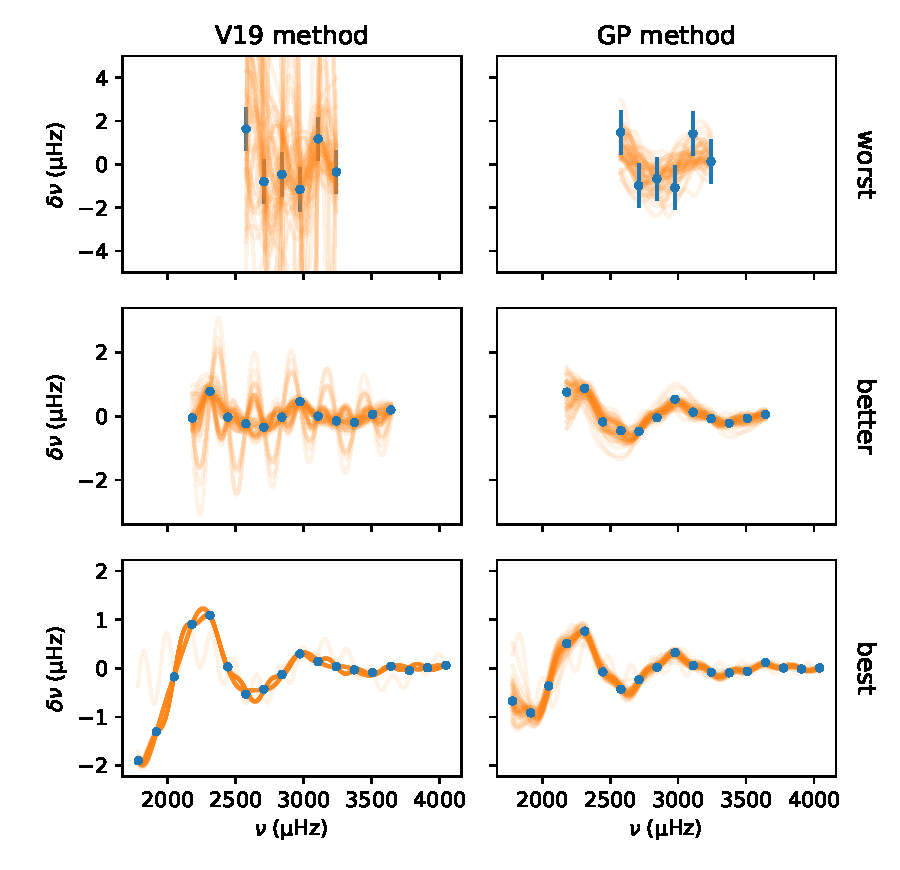
\includegraphics{figures/glitch-test-signal.pdf}
    \caption[50 random draws from the V19 and GP results showing the total glitch signal as a function of frequency.]{50 random draws from the V19 and GP methods showing the total glitch signal, \(\delta\nu = \delta_\helium(\nu) + \delta_\bcz(\nu)\), as a function of frequency, \(\nu\). The data points plot in blue are the median smooth component model at \(\vect{n}\), subtracted from the observed modes (\(\vect{\nu}_\obs\)) with their observed uncertainty (\(\sigma_\obs\)).}
    \label{fig:glitch-test-signal}
\end{figure}

In Figure \ref{fig:glitch-test-signal}, we plot the predicted total glitch component (\(\delta\nu\)) using 50 draws from the posterior distribution for both methods. We subtracted the median smooth component (\(\tilde{f}(n)\)) from the observed \(\nu_n\) over-plot. For each scenario, both methods predicted similar glitch components. However, the \citetalias{Verma.Raodeo.ea2019} method showed more extreme multimodality in all cases. For example, the better case showed a high-amplitude (\(\sim \SI{2}{\micro\hertz}\)) BCZ glitch solution which is not present with the GP method. Such a large BCZ signature would be unlikely. Additionally, the two methods differed by \(\sim \SI{1}{\micro\hertz}\) at low frequency in the best case. Despite this, the \citetalias{Verma.Raodeo.ea2019} method appeared to be more confident in its glitch solutions compared to the GP method.

\begin{figure}[!tb]
    \centering
    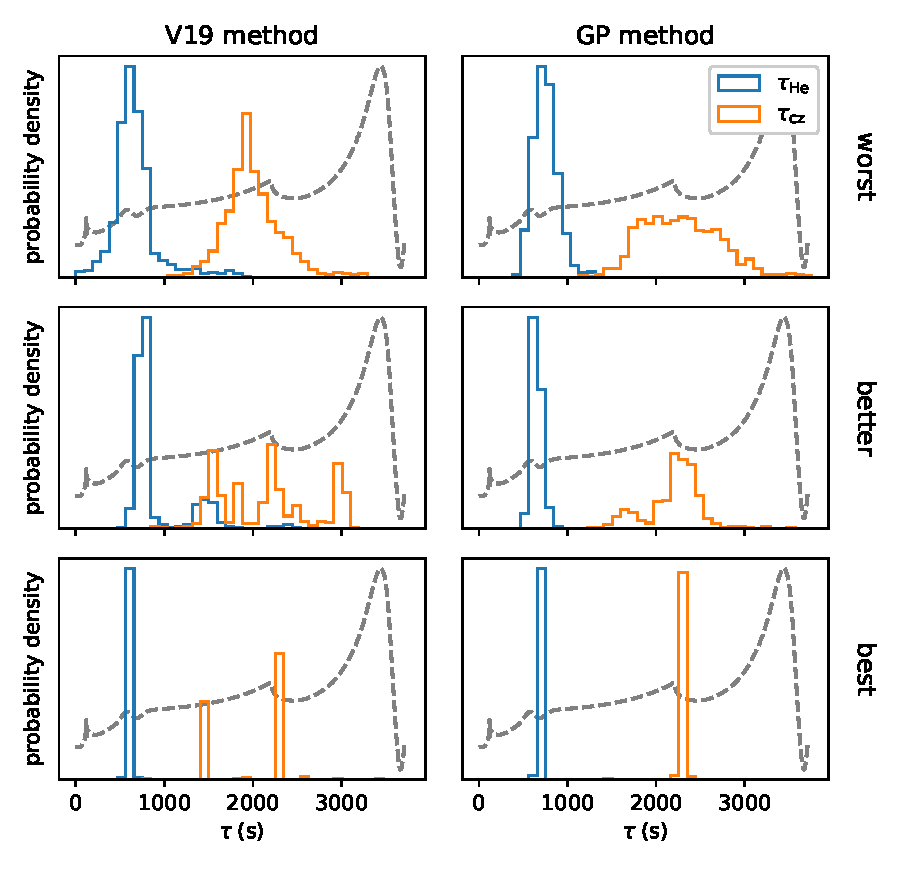
\includegraphics{figures/glitch-test-tau.pdf}
    \caption[Samples from the V19 and GP methods for the acoustic depths of the helium glitch (\(\tau_\helium\)) and base of the convective zone (\(\tau_\bcz\))]{Samples from the V19 and GP methods for the acoustic depths of the helium glitch (\(\tau_\helium\)) and base of the convective zone (\(\tau_\bcz\)). The sound-speed gradient from Figure \ref{fig:sound-speed-gradient} is over-plot with a grey dashed line.}
    \label{fig:glitch-test-tau}
\end{figure}

In Figure \ref{fig:glitch-test-tau}, we plotted posterior distributions for the glitch acoustic depths, \(\tau_\helium\) and \(\tau_\bcz\), and compared them to the sound speed gradient of the test star from Figure \ref{fig:sound-speed-gradient}. We expect the acoustic depths to approximately line up with the sharp structural changes. For the worst case, both methods gave broad distributions for the acoustic depths, compatible with their respective initial guesses and priors. The \citetalias{Verma.Raodeo.ea2019} method initial guesses appeared to underestimate \(\tau_\bcz\), whereas the GP method prior was broad enough to encompass a wide range of possible \(\tau_\bcz\). In the better and best cases, we found that the \citetalias{Verma.Raodeo.ea2019} solutions were multimodal. For example, the better case found solutions for \(\tau_\helium\) far deeper into the star than we would expect, at around \SI{1500}{\second} and \SI{2500}{\second}.

% As predicted by \citet{Houdek.Gough2007} and shown in \citet{Verma.Faria.ea2014}... This is because \(\delta\nu_\helium\) does not include the smaller glitch component due to the first ionisation of helium, located at a smaller \(\tau\).
The values for \(\tau_\helium\) obtained were under-predicted compared to the location of the trough due to the second ionisation of helium. We can see this for the best star fit with the \citetalias{Verma.Raodeo.ea2019} method which finds \(\tau_\helium = \SI{619(15)}{\second}\). The depression in \(\gamma\) due to He\,\textsc{ii} ionisation in the respective stellar model is located at \SI{733}{\second}. On the other hand, the GP method was closer with \(\tau_\helium = \SI{696(19)}{\second}\).

\begin{figure}[tb]
    \centering
    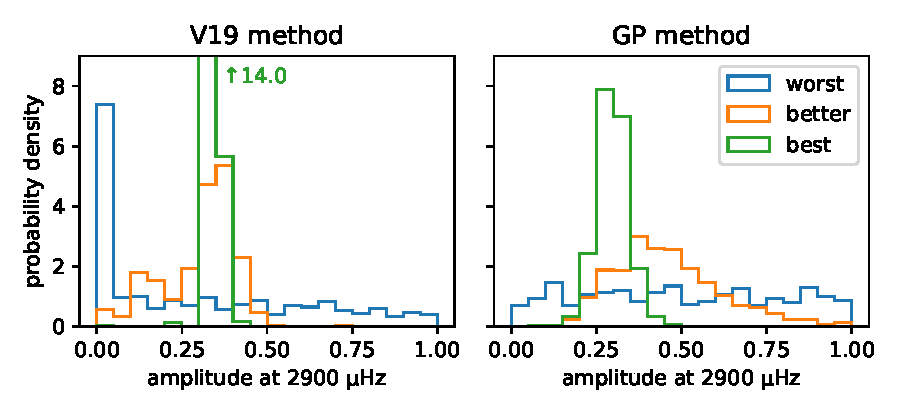
\includegraphics{figures/glitch-test-amplitude.pdf}
    \caption[Samples of the helium glitch amplitude at a reference frequency of \SI{3000}{\micro\hertz} fit with the V19 and GP methods for the worst, better, and best case test data.]{Samples of the helium glitch amplitude at a reference frequency of \SI{3000}{\micro\hertz} fit with the V19 and GP methods for the worst, better, and best case test data. The tallest bar in the V19 method panel is cropped with its value displayed in green text.}
    \label{fig:glitch-test-amplitude}
\end{figure}

We compared helium glitch amplitudes at \(\nu_\mathrm{ref}\) from both methods in Figure \ref{fig:glitch-test-amplitude}. The \citetalias{Verma.Raodeo.ea2019} method preferred low-amplitude solutions for the worst and better cases compared to the GP method. On the other hand, the GP method reflected our prior in the worst case, with the width of the distribution shrinking as the data improved. The GP method did show some bi-modality in the better case, with higher solutions at \(A_\helium^\mathrm{ref} \approx 0.7\) which were not found by the \citetalias{Verma.Raodeo.ea2019} method. In the best case, the \citetalias{Verma.Raodeo.ea2019} method obtained \(A_\helium^\mathrm{ref} = 0.347_{-0.005}^{+0.006}\), whereas the GP method found \(A_\helium^\mathrm{ref} = 0.296_{-0.036}^{+0.042}\).

% Why not use delta gamma / gamma as the probe of helium abundance? That is proportional to alpha / sqrt(beta). Then, an update to this method can use this and beta as a parameter and then work out alpha from that, since beta should scale with tau and the depth is a signature of helium abundance. Be careful as number of modes correlates with delta nu value of fit.

\subsection{16 Cyg A}

We compared the results from both methods applied to the 16 Cyg A data in Figure \ref{fig:glitch-16cyga}. We found that the \citetalias{Verma.Raodeo.ea2019} method predicted extreme solutions for the glitch where the GP method did not. There was also a difference of about \SI{1}{\micro\hertz} at the low frequency end such that the \citetalias{Verma.Raodeo.ea2019} predicted a larger glitch amplitude. Otherwise, the two methods gave similar solutions for the glitch function.

Both methods found similar values for \(\tau_\helium\) but relatively different distributions for \(\tau_\bcz\). Regarding the helium glitch, the \citetalias{Verma.Raodeo.ea2019} method found \(\tau_\helium = 917_{-53}^{+50} \, \mathrm{s}\), and our GP method obtained \(\tau_\helium = 931_{-88}^{+59} \, \mathrm{s}\), within 1-\(\sigma\) of each other. Similarly to the test star, the GP method found a slightly larger value of \(\tau_\helium\) than the \citetalias{Verma.Raodeo.ea2019} method. \citet{Verma.Faria.ea2014} fit the glitch using \(l=0,1,2\) modes and found an acoustic depth of \SI{930(14)}{\second}, within 1-\(\sigma\) of both methods in this work.

We calculated the helium glitch amplitude at a reference frequency of \SI{2188.5}{\micro\hertz}, equivalent to \(\nu_{\max}\) obtained by \citet{Lund.SilvaAguirre.ea2017}. Samples from both posteriors are shown in the bottom panel of Figure \ref{fig:glitch-16cyga}. We found \(A_\helium^\mathrm{ref} = 0.260_{-0.065}^{+0.050}\,\si{\micro\hertz}\) for the \citetalias{Verma.Raodeo.ea2019} method, and \(A_\helium^\mathrm{ref} = 0.333_{-0.073}^{+0.081}\,\si{\micro\hertz}\) for the GP method. Both values were about 1-\(\sigma\) apart. Additionally, both methods found \(A_\bcz^\mathrm{ref} \sim 0.1\,\si{\micro\hertz}\), with the GP method favouring a smaller value. The \citetalias{Verma.Raodeo.ea2019} method found some solutions where \(A_\bcz^\mathrm{ref}\) was larger than \(A_\helium^\mathrm{ref}\), something we would not expect because the modes are less sensitive to structural changes deeper in the star.

\begin{figure}[!tb]
    \centering
    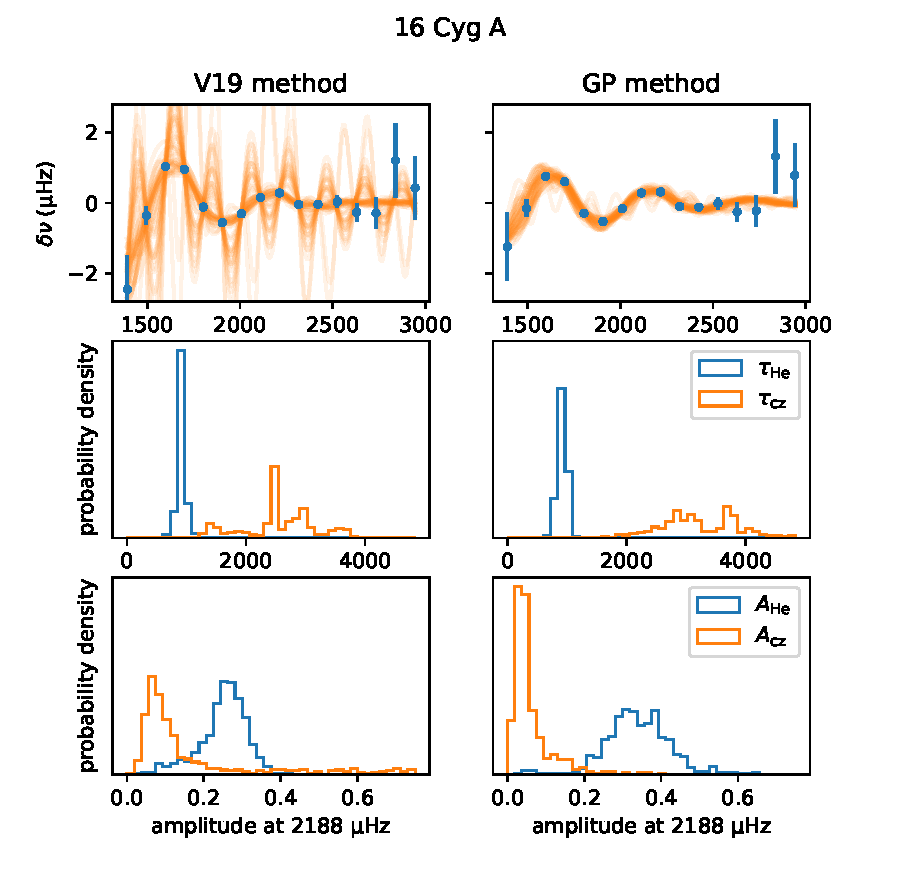
\includegraphics{figures/glitch-16cyga.pdf}
    \caption[Results for the glitch fit to 16 Cyg A using the V19 method and GP method.]{Results for the glitch fit to 16 Cyg A using the \citetalias{Verma.Raodeo.ea2019} method (\emph{left}) and GP method (\emph{right}). The top panel shows 50 draws from the posterior prediction of \(\delta\nu = \delta\nu_\helium + \delta\nu_\bcz\) with the observed \(\nu_n\) minus the median smooth background component of the model. The middle and bottom panels shows the posterior sample probability density for the acoustic depths and reference amplitudes of the glitches respectively.}
    \label{fig:glitch-16cyga}
\end{figure}

\section{Discussion}\label{sec:glitch-disc}

% Discuss major differences

\begin{figure}[tb]
    \centering
    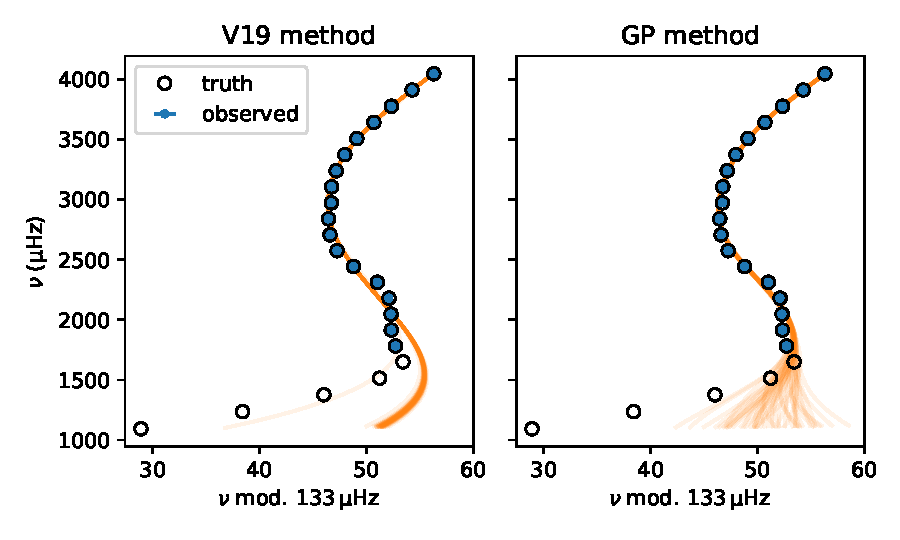
\includegraphics{figures/glitch-test-smooth.pdf}
    \caption[Echelle-like diagrams showing mode frequencies plot against their frequency modulo \SI{133}{\micro\hertz} for the best case scenario.]{Echelle-like diagrams showing mode frequencies plot against their frequency modulo \SI{133}{\micro\hertz} for the best case scenario. The orange lines show 50 draws from the model posterior predictions with the glitch component removed (\(f(n) - \delta\nu\)) for both methods. The predictions are made from a lower radial order \(n=8\) than the observed modes. The true values from model R are shown for each mode. Some radial orders (\(n\)) are shown next to the modes for context.}
    \label{fig:best-smooth}
\end{figure}

Throughout this work, we found a smaller \(\delta\nu\) amplitude at low frequency with the GP method than with the \citetalias{Verma.Raodeo.ea2019} method. This was particularly visible in the best case and in 16 Cyg A. We expected this was a result of the different smooth background models. In Figure \ref{fig:best-smooth} we plotted the smooth component of each model extended to lower order, unobserved modes. We found the GP background component had a turning point at \(\nu \approx \SI{1900}{\micro\hertz}\), higher than the \citetalias{Verma.Raodeo.ea2019} method at \(\nu \approx \SI{1500}{\micro\hertz}\). The smooth component of the \citetalias{Verma.Raodeo.ea2019} method was confidently incorrect outside the observed frequencies. Conversely, the GP method predicted closer to the truth with increasing uncertainty further from the observations. It appeared that the GP provided a more accurate representation of the underlying function than the polynomial.

\begin{figure}[!tb]
    \centering
    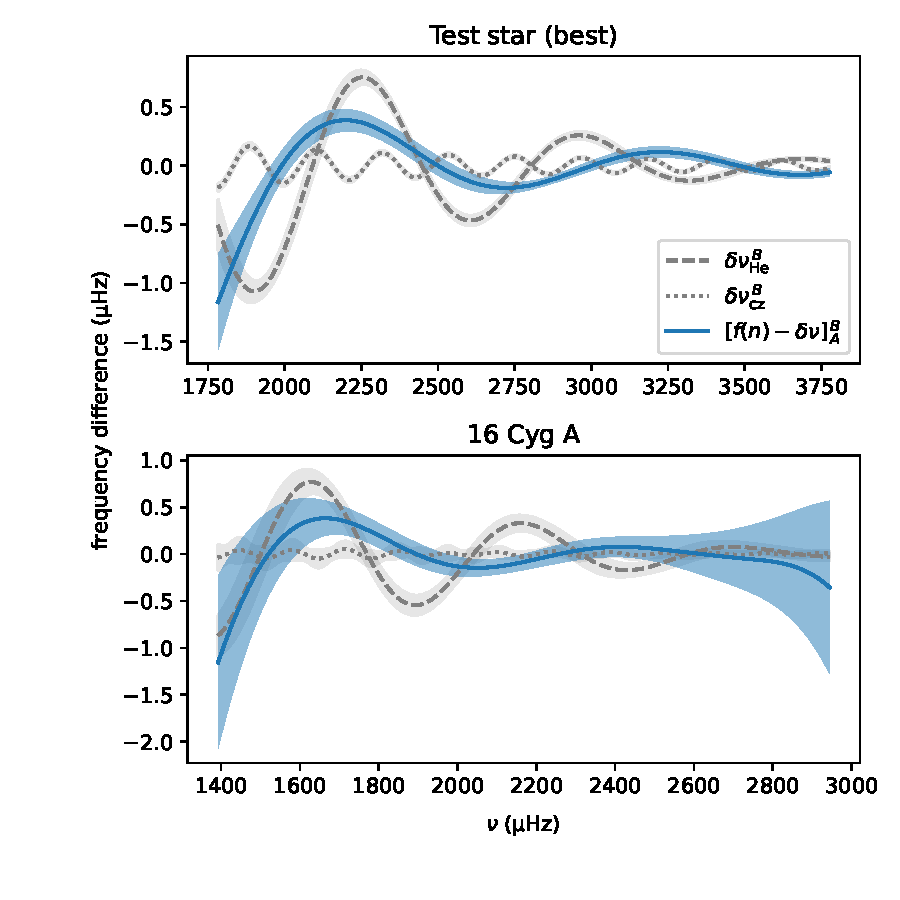
\includegraphics[trim={0.4in 0.2in 0 0},clip]{figures/glitch-res.pdf}
    \caption[The difference between the model without the glitch components predicted by theV19 method and the GP method.]{The difference between the model without the glitch components (\(f(n) - \delta\nu\)) predicted by the \citetalias{Verma.Raodeo.ea2019} method (A) and the GP method (B). The glitch components from the GP method are plot in grey for context. The 68 per cent confidence region is shaded for each line.}
    \label{fig:smooth-res}
\end{figure}

In the test star's best case and 16 Cyg A, the GP method found a higher \(\tau_\helium\) than the \citetalias{Verma.Raodeo.ea2019} method. This could be because the GP was better able to distinguish between the He\,\textsc{ii} glitch and the smaller He\,\textsc{i} glitch. To explore this, we plotted the difference between each model's predictions for the smooth component in Figure \ref{fig:smooth-res}. We saw a clear periodic signal in the differences. The period of this signal in the test star corresponded to an acoustic depth of \(\sim \SI{500}{\second}\), matching the location of He\,\textsc{i} ionisation in model R. The periodic signal was less pronounced for 16 Cyg A, but corresponded to a plausible He\,\textsc{i} acoustic depth of \(\sim \SI{700}{\second}\). We expected that the polynomial was not flexible enough to pick up the He\,\textsc{i} ionisation signature, hence lowering its mean value for \(\tau_\helium\).

% Discuss the prior

The \citetalias{Verma.Raodeo.ea2019} method found several extreme solutions for \(\delta\nu\) whereas GP method did not. We expected this because the GP method used a prior over the model parameters. We tested relaxing the prior on \(\vect{\theta}_B\) and found similar multimodal posteriors to the \citetalias{Verma.Raodeo.ea2019} method. This showed that the prior helped eliminate unrealistic solutions. However, care should be taken over the choice of prior on \(\vect{\theta}_B\) to realistically reflect our expectation. If some of our prior assumptions are incorrect, they may bias the results. For example, the outer convective region gets shallower as stars get hotter (approaching \(\teff \approx \SI{7000}{\kelvin}\)) making the assumption that \(\tau_\bcz/\tau_0 \approx 0.6\) an overestimate in these cases. We accommodate for this with a wide prior on \(\tau_\bcz\), but our prior could be more informed. There is a notable temperature dependence to \(\tau_\bcz/\tau_0\) observed in the grid of stellar models which could be exploited in the future when constructing the prior.

Additionally, the joint posteriors for \(\alpha_\helium\) and \(\beta_\helium\) were correlated in both methods. This was expected, because larger values of \(\beta_\helium\) can be compensated for with a larger amplitude factor (\(\alpha_\helium\)). In the GP method, we did not include this expected correlation in our prior. Hence, we found that having broader priors on \(\alpha_\helium\) and \(\beta_\helium\) lead to the prior predicting unrealistic glitches. We could account for this by using a multivariate prior for the amplitude parameters. Despite this, our approach still improves on the \citetalias{Verma.Raodeo.ea2019} method by using a prior in the first place.

A potential limitation of the GP method is that we calculate the glitch at \(\tilde{f}_B(n)\) from the linear asymptotic equation (Equation \ref{eq:asy}). In regions where the gradient of \(\delta\nu\) is high, the difference between \(\tilde{f}_B(n)\) and the true frequency can be up to \(\sim \SI{0.1}{\micro\hertz}\). Our choice of kernel function cannot absorb this difference because is varies on a short length-scale. Instead, we accounted for this uncertainty by adding Gaussian noise to the model parametrised by \(\sigma\). However, for the best test star, we found \(\sigma \approx 0.05\), which was larger than the observational uncertainty, \(\sigma_\obs = 0.01\). This could limit our method's inference ability for the best asteroseismic targets. One solution is to replace \(\tilde{f}_B(n)\) with a quadratic \citep[e.g.][]{Nielsen.Davies.ea2021} which better approximates \(\nu_n\). However, the GP kernel would need to be adjusted to account for this.

% Using the glitch parameters as a helium diagnostic could involve measuring the amplitude of the helium glitch at a reference frequency such as \(\nu_{\max}\). We should expect solutions for this reference amplitude (\(A_\mathrm{ref}\)) to converge on a value as the data quality increases from worst to best. It is also important that the uncertainty of the reference amplitude is accurate if using it to constrain helium abundance in a population of stars. If using V19 method on a population of stars, this could bias inference towards lower values of helium abundance.

\section{Conclusion}

We introduced a new method for modelling acoustic glitches in solar-like oscillators using a Gaussian Process. Testing the method on a model star, we found that it more accurately characterised the underlying, smoothly-varying functional form of the radial modes than the 
\citetalias{Verma.Raodeo.ea2019} method. Furthermore, our method appeared able to absorb the glitch component from He\,\textsc{i} ionisation, for which the polynomial was not flexible enough. However, this questions whether the He\,\textsc{i} ionisation glitch should be explicitly included in the model.

Additionally, the GP method provided more believable uncertainties on the glitch parameters, whereas the \citetalias{Verma.Raodeo.ea2019} method was over-confident with the best data and under-confident with the worst. Robust uncertainties are important when using the results to make further inference about helium enrichment. In this case, the GP marginalised over correlated noise in the model, not possible with the \citetalias{Verma.Raodeo.ea2019} method.

Future development of the method could involve building a prior for the glitch parameters. For example, we could start with fitting the model to simulated stars and using the results to build an empirical prior. Then, we could run the model on a larger asteroseismic sample of main sequence stars \citep[e.g.][]{Lund.SilvaAguirre.ea2017,Davies.SilvaAguirre.ea2016} and compare our results to those from \citet{Verma.Raodeo.ea2019}. Additionally, we could add parameters from the GP model to the hierarchical model introduced in \citet{Lyttle.Davies.ea2021}. Ultimately, our goal is to scale this method in anticipation of the \(\sim 10^4\) solar-like oscillators expected to be observed by \emph{PLATO} \citep{Rauer.Catala.ea2014}.
